\documentclass[12pt,reqno, twoside]{amsbook}
%%%%%%%%%%%%%%%%%%%%%%%%%%%%%%%%%%%%%%%%%%%%%%%%%%%%%%%%%%%%%%%%%%%%%%%%%%%%%%%%%%%%%%%%%%%%%%%%%%%%%%%%%%%%%%%%%%%%%%%%%%%%%%%%%%%%%%%%%%%%%%%%%%%%%%%%%%%%%%%%%%%%%%%%%%%%%%%%%%%%%%%%%%%%%%%%%%%%%%%%%%%%%%%%%%%%%%%%%%%%%%%%%%%%%%%%%%%%%%%%%%%%%%%%%%%%
\usepackage{eurosym}
\usepackage{amsmath}
\usepackage{amssymb}
\usepackage{amsfonts}
\usepackage[onehalfspacing]{setspace}
\usepackage{chngcntr}
\usepackage{graphicx}
\usepackage[a4paper, margin=2.5cm]{geometry}
\usepackage[english]{babel}
\usepackage{fancyhdr}
\usepackage{titlesec}
\usepackage{enumitem}
\usepackage{etoolbox}
\usepackage{csquotes}
\usepackage[printonlyused]{acronym}
\usepackage{hyperref}
\usepackage{booktabs}
\usepackage{multirow}
\usepackage{longtable}
\usepackage{tabularx}
\usepackage{tikz}
\usetikzlibrary{positioning}
%
% you may need to uncomment the command below if you use eps format for figures
%\usepackage{epstopdf}
%
\usepackage[
    backend=biber,
    style=ieee,
  ]{biblatex}
\addbibresource{references.bib}
%
\makeatletter
    \def\section{\@startsection{section}{1}%
      \z@{.5\linespacing\@plus.7\linespacing}{.25\linespacing}%
      {\normalfont\bfseries\flushleft}}
    \def\subsection{\@startsection{subsection}{2}%
      \z@{.5\linespacing\@plus.7\linespacing}{.25\linespacing}%
      {\normalfont\bfseries\flushleft}}
%
\makeatother
\setcounter{MaxMatrixCols}{10}
%
\providecommand{\U}[1]{\protect\rule{.1in}{.1in}}
\theoremstyle{plain}
\newtheorem{acknowledgement}{Acknowledgement}
\newtheorem{algorithm}{Algorithm}[chapter]
\newtheorem{axiom}{Axiom}[chapter]
\newtheorem{case}{Case}[chapter]
\newtheorem{claim}{Claim}[chapter]
\newtheorem{conclusion}{Conclusion}[chapter]
\newtheorem{condition}{Condition}[chapter]
\newtheorem{conjecture}{Conjecture}[chapter]
\newtheorem{corollary}{Corollary}[chapter]
\newtheorem{criterion}{Criterion}[chapter]
\newtheorem{definition}{Definition}[chapter]
\newtheorem{example}{Example}[chapter]
\newtheorem{exercise}{Exercise}[chapter]
\newtheorem{lemma}{Lemma}[chapter]
\newtheorem{notation}{Notation}[chapter]
\newtheorem{problem}{Problem}[chapter]
\newtheorem{proposition}{Proposition}[chapter]
\newtheorem{remark}{Remark}[chapter]
\newtheorem{solution}{Solution}[chapter]
\newtheorem{summary}{Summary}[chapter]
\newtheorem{theorem}{Theorem}[chapter]
\numberwithin{equation}{chapter}
%
\makeatletter
\newcommand\frontFont{\@setfontsize\frontFont{14.4}{14.4}}
\makeatother
%
% Please write the references according to your school
%
\newenvironment{dedication}
  {%\clearpage           % we want a new page
   \thispagestyle{empty}% no header and footer
   \vspace*{\stretch{1}}% some space at the top
   \itshape             % the text is in italics
   \raggedleft          % flush to the right margin
  }
  {\par % end the paragraph
   \vspace{\stretch{3}} % space at bottom is three times that at the top
   %\clearpage           % finish off the page
  }
  \numberwithin{section}{chapter}
\fancyhead{}
\fancyfoot{}
\pagestyle{fancy}
\fancyfoot[LE,RO]{\thepage}
%
\makeatletter
\def\ps@plain{\ps@empty
 \def\@evenfoot{%
   \normalfont\scriptsize
   \rlap{\thepage}\hfil
   }%
 \def\@oddfoot{%
   \normalfont\scriptsize \hfil
   \llap{\thepage}}%
}
\makeatother
\renewcommand{\headrulewidth}{0pt}
\renewcommand{\footrulewidth}{0pt}
%
\usepackage{montserrat}
\usepackage[T1]{fontenc}
\renewcommand*\oldstylenums[1]{{\fontfamily{Montserrat-TOsF}\selectfont #1}}
%
\numberwithin{table}{chapter}
\numberwithin{figure}{chapter}
%
%%% PT: BEGIN
% \addto\captionsenglish{\renewcommand{\chaptername}{Capítulo}}
% \addto\captionsenglish{\renewcommand{\tablename}{Tabela}}
% \addto\captionsenglish{\renewcommand{\figurename}{Figura}}
% \addto\captionsenglish{\renewcommand{\figurename}{Figura}}
% \addto\captionsenglish{\renewcommand{\contentsname}{Conteúdo}}
% \addto\captionsenglish{\renewcommand{\listfigurename}{Lista de Figuras}}
% \addto\captionsenglish{\renewcommand{\listtablename}{Lista de Tabelas}}
% \DeclareDelimFormat{finalnamedelim}{\addspace e\space}
%%% PT: END
%
\begin{document} %%%%%%%%%%%%%%%%%%%%% BEGIN %%%

\sffamily
\frontFont
\begin{flushleft}
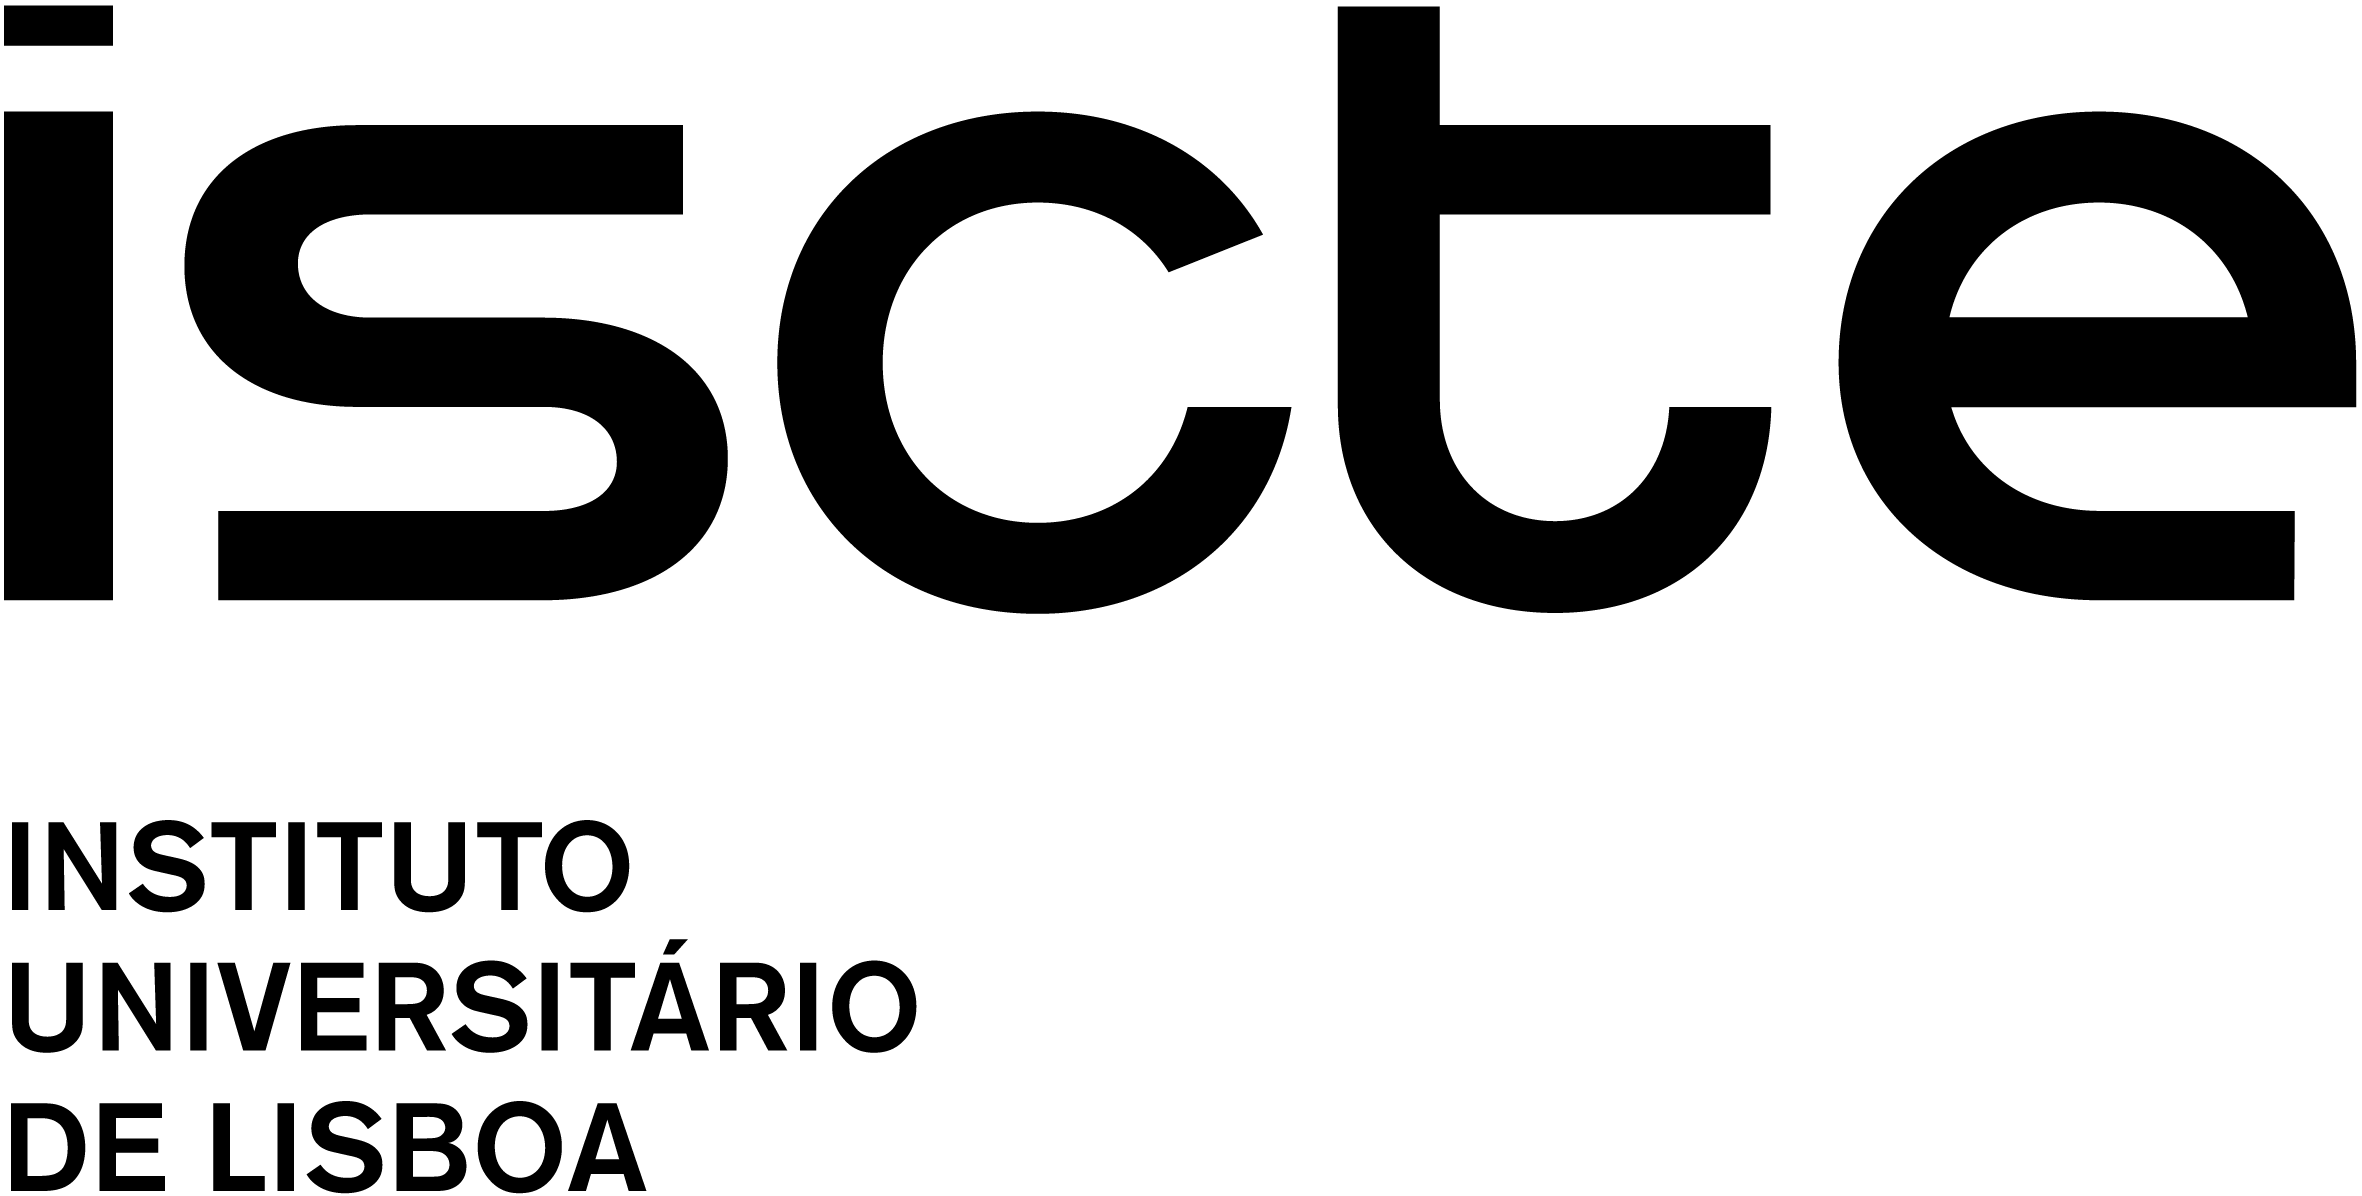
\includegraphics[width=6.03cm]{imagens/iscte}\\[3.3mm]

\hrulefill
~\\
~\\
~\\
\textbf{Título}\\
~\\
~\\
~\\
~\\
\textit{name}\\
~\\
~\\
~\\
Master in Computer Engineering\\
~\\
~\\
~\\
Supervisor:\\
Doctor \textit{name}, \textit{category} Professor,\\
Iscte -- Instituto Universitário de Lisboa\\
~\\
~\\
~\\
Co-Supervisor:\\
Doctor \textit{name}, \textit{category} Professor,\\
\textit{instituição}\\
~\\
~\\
~\\
~\\
October, 2022
\end{flushleft}
\thispagestyle{empty}
\cleardoublepage
\begin{flushleft}
  
\includegraphics[width=6.03cm]{imagens/ista}\\[7mm]
\hrulefill
~\\
~\\
~\\
Department of Information Science and Technology\\
~\\
~\\
\textbf{Título}\\
~\\
~\\
~\\
~\\
\textit{name}\\
~\\
~\\
~\\
Master in Computer Engineering\\
~\\
~\\
~\\
Supervisor:\\
Doctor \textit{name}, \textit{category} Professor,\\
Iscte -- Instituto Universitário de Lisboa\\
~\\
~\\
~\\
Co-Supervisor:\\
Doctor \textit{name}, \textit{category} Professor,\\
\textit{university}\\
~\\
~\\
~\\
~\\
October, 2022
  \end{flushleft}
  \thispagestyle{empty}
\rmfamily
\normalsize
\frontmatter
%\addtocontents{toc}{\setcounter{tocdepth}{2}}
\thispagestyle{empty}

\frontmatter
\addtocontents{toc}{\setcounter{tocdepth}{2}}
\thispagestyle{empty}

\begin{dedication}%

\begin{flushright}
\textit{Write here your dedication}
\end{flushright}%
\end{dedication}

\setcounter{page}{1}
\pagenumbering{roman} %
\chapter*{Acknowledgment}

Write here the acknowledgments and grants, if any

\chapter*{Resumo}

Escrever aqui o resumo em Português.

\vspace{3ex}
\textsc{Palavras Chave:} \textit{palavra\_1}, \textit{palavra\_2}, \dots

\chapter*{Abstract}

Write here your abstract in English.

\vspace{3ex}
\textsc{Keywords:} \textit{word\_1}, \textit{word\_2}, \dots

\tableofcontents
\listoffigures
\listoftables
\cleardoublepage
%\printglossary[type=\acronymtype, nonumberlist, nogroupskip]
\chapter*{List of Acronyms}
\begin{acronym}
 \acro{AI}{Artificial Intelligence}
 \acro{BIoT}{Blockchain-based Internet of Things}
 \acro{C2DTA}{Consumer-Controlled Digital Twin Architecture}
 \acro{C2PDT}{Consumer-Controlled Personal Digital Twin}
 \acro{CID}{Content Identifier}
 \acro{DGA}{Data Governance Act}
 \acro{DID}{Decentralized Identifier}
 \acro{DIDComm}{Decentralized Identifier Communication}
 \acro{DLT}{Distributed Ledger Technology}
 \acro{DSR}{Design Science Research}
 \acro{DT}{Digital Twin}
 \acro{EGW}{Edge Gateway}
 \acro{FSD}{Full Self-Driving}
 \acro{GDPR}{General Data Protection Regulation}
 \acro{HSM}{Hardware Security Module}
 \acro{IDC}{International Data Corporation}
 \acro{IDS}{International Data Spaces}
 \acro{IoT}{Internet of Things}
 \acro{IPFS}{InterPlanetary File System}
 \acro{M2M}{Machine-to-Machine}
 \acro{ML}{Machine Learning}
 \acro{MQTT}{Message Queuing Telemetry Transport}
 \acro{OEM}{Original Equipment Manufacturer}
 \acro{PDE}{Personal Data Ecosystem}
 \acro{PDS}{Personal Data Store}
 \acro{PDT}{Personal Digital Twin}
 \acro{PRISMA}{Preferred Reporting Items for Systematic Reviews and Meta-Analyses}
 \acro{SD}{Smart Device}
 \acro{SLR}{Systematic Literature Review}
 \acro{SSI}{Self-Sovereign Identity}
 \acro{TD}{Thing Description}
 \acro{TLS}{Transport Layer Security}
 \acro{TPM}{Trusted Platform Module}
 \acro{VC}{Verifiable Credential}
 \acro{VDR}{Verifiable Data Registry}
 \acro{VP}{Verifiable Presentation}
 \acro{W3C}{World Wide Web Consortium}
 \acro{WoT}{Web of Things}
\end{acronym}

\mainmatter

\hyphenation{wri-te he-re pro-per hy-phe-ni-za-tion
}%

\setcounter{page}{1} \pagenumbering{arabic}

% ============================================================
%  Chapter 1 — Introduction
% ============================================================
\chapter{Introduction}
\label{ch:introduction}

\noindent The International Data Corporation (IDC)~\cite{idc:2021} estimates that by 2025, \ac{IoT} devices---encompassing machines, sensors, and cameras---will collectively generate 79.4~zettabytes of data.
Although \acp{SD} can increase consumer well-being~\cite{lee:lee:2020}, they also present significant challenges.
Sensors invade the consumer privacy sphere, capturing data stored in silos that attract cybercriminals~\cite{weber:2010}, while \acp{OEM} often exploit these data for their own benefit~\cite{zuboff:2019}, leaving consumers without tangible rewards~\cite{spiekermann:korunovska:2017}.
The framework governing the collection and use of personal data involving consumers and \acp{OEM} to create economic value, known as the \ac{PDE}~\cite{world:economic:forum:2011}, is unbalanced~\cite{ctrl:shift:2014}.
It allows \acp{OEM} to monopolize data-flow profits while consumers bear the system's externalities, and is therefore associated with a loss of control over personal information~\cite{abiteboul:andre:abiteboul:2015}.

To address this imbalance, industry and academia are exploring blockchain-based \ac{IoT} solutions for people-centered architectures~\cite{samaniego:deters:2017}.
Blockchain's strong cryptographic foundation, immutable and tamper-proof nature, decentralization, and smart-contract support allow for critical mechanisms that, when integrated with user-centered architectures, elevate consumer status in the \ac{PDE}~\cite{zyskind:nathan:pentland:2015}.
By leveraging blockchain \ac{DLT}, it is possible to establish a network of trustless peers that collectively agree on an immutable, auditable, and cryptographically secure shared version of the truth~\cite{zheng:xie:dai:chen:wang:2018}.
This network offers support for decentralized identifiers that link users with their data without the need for third parties~\cite{muhle:suhr:zanker:meinel:2018}.
When combined with Personal Data Stores, frameworks that allow users to collect, store, manage, and share their data according to their preferences~\cite{deangelis:pieri:2019}, this identity mechanism, referred to as \ac{SSI}~\cite{preukschat:reed:2021}, gives consumers sovereign control over their data.
When used within a user-centered framework, this mechanism transforms consumers from passive data subjects to active participants in the \ac{PDE}, underscoring the critical role of maintaining data rights---access, usage, and sharing---firmly in the hands of consumers~\cite{janssen:brous:estevez:barbosa:2018}.

The \ac{DT} concept originated at NASA and became publicly recognized in 2003~\cite{grieves:2014}.
It refers to a virtual representation or digital counterpart of a physical object, system, or process~\cite{minerva:lee:crespi:2020}.
Since its introduction, the concept has evolved and matured, reaching a significant growth stage by 2014~\cite{grieves:vickers:2017}.
Transforma Insights~\cite{transforma:insights:2021} forecasts a market size of 24.1~billion devices and a reach of \$1.5~trillion, with the consumer sector accounting for 65\% of all connections.
\ac{DT} reframes much of the early efforts to develop connected-device solutions, initially based on telemetry and \ac{M2M} communications and later enhanced with \ac{IoT} technologies~\cite{madakam:ramaswamy:tripathi:2015}.
This evolution has produced a more structured, multifaceted development framework supporting services and \ac{AI}~\cite{minerva:lee:crespi:2020}.
For instance, a smartwatch with a \ac{DT} extends beyond basic data collection: it continuously gathers and analyzes detailed data to update and refine its virtual model, creating a comprehensive understanding of the user's behaviors, activities, and physiological states.

As \ac{DT} crosses into the consumer realm, it is reasonable to surmise that some \acp{OEM} may exploit the concept of product personalization~\cite{thiesse:2007} or other features with disproportionately lower impact for consumers to gain further consumer insights with \ac{DT}-based solutions.
Therefore, it is vital to develop mechanisms that enable consumers to control their devices' \acp{DT}~\cite{kopponen:hahto:kettunen:etal:2022}.
Tesla is a paradigmatic example of the urgent need for such mechanisms: its trillion-dollar valuation~\cite{tesla:marketcap:2024} is supported by its ability to leverage \acp{DT} to train its Full Self-Driving feature~\cite{karpathy:matroid:2020,tesla:ai:day:2021}.

%--------------------------------------------------------------
\section{Problem Statement}
\label{sec:problem}
%--------------------------------------------------------------

\noindent The economic fairness challenge in controlling \acp{DT} arises from the current cloud-based approach, where \acp{OEM} retain \emph{de facto} control over the \ac{DT} and the associated consumer-generated data~\cite{hummel:braun:dabrock:2021}.
As consumers become more aware of the growing value of data, they are likely to demand solutions that restore control and ensure equitable participation.

Furthermore, proponents of edge computing, federated learning, and privacy-preservation methods such as homomorphic encryption emphasize the benefits of storing and processing data at the edge as a mechanism to improve the privacy and security of \ac{AI} training data within \ac{IoT} contexts~\cite{idc:ai:2024,shi:cao:zhang:li:xu:2016,mcmahan:moore:ramage:hampson:arcas:2017,yang:liu:chen:tian:2019,li:sahu:talwalkar:smith:2020}.
However, these works often overlook the critical step of ensuring that data are kept at the edge in a self-sovereign manner under consumer control.

This dissertation addresses these challenges by presenting the \ac{C2DTA}.
The main objective of \ac{C2DTA} is to empower consumers in the \ac{PDE} by shifting the \ac{DT} from the cloud under \ac{OEM} control to the edge under consumer control~\cite{spiekermann:korunovska:boenisch:2019}.
This shift makes consumers \emph{de facto} controllers---meaning they have actual control in practice~\cite{finck:2018}---of their \ac{SD} data by giving them effective control over the \ac{DT} and its associated data~\cite{de:hert:papakonstantinou:2016}.

\ac{C2DTA} addresses two key challenges:
\begin{enumerate}
    \item \textbf{Economic fairness through the control of \acp{DT}.} The current cloud-based approach allows \acp{OEM} to retain \emph{de facto} control over the \ac{DT} and associated consumer-generated data. \ac{C2DTA} restores consumer sovereignty by hosting the \ac{DT} at the edge.
    \item \textbf{Bridging the edge-computing gap.} \ac{C2DTA} provides the practical foundation necessary for self-sovereign, edge-based data management, closing the gap between proposals for edge computing, federated learning, and privacy-preserving technologies and their actionable implementation.
\end{enumerate}

%--------------------------------------------------------------
\section{Research Objectives}
\label{sec:objectives}
%--------------------------------------------------------------

\noindent Building on the problem statement, this dissertation pursues the following research objectives:

\begin{description}
    \item[RO1.] \textbf{Self-sovereign \ac{DT} ecosystem architecture.} Propose an architecture that enables stakeholders of the digital-twinned \ac{SD} ecosystem to securely manage \acp{DT} and leverage their data. In this architecture, those who own devices control the associated \acp{DT} at the edge, and stakeholders transact in a decentralized, self-sovereign, and secure manner.

    \item[RO2.] \textbf{\ac{DT}, \ac{SSI}, and blockchain integration taxonomy.} Propose a structured framework for consistently evaluating conceptual and practical implementations, enabling clear classification, identifying research gaps, and guiding future development in decentralized systems.

    \item[RO3.] \textbf{Hyperledger Fabric, Indy, and Aries integration.} Propose an architecture that integrates Hyperledger Fabric for managing \acp{SD} and datasets with Hyperledger Aries for overseeing stakeholder identifiers, \acp{VC}, and secure communication protocols through ACA-Py. This integration encompasses eight detailed use cases across the full \ac{SD} lifecycle---manufacturing, sale, ownership transfer, twinning, and untwinning.

    \item[RO4.] \textbf{Future innovation for consumer empowerment.} Introduce concepts emerging from the architecture, including ``data-only \acp{DT}'' and the aggregation of several consumer-controlled \acp{DT} into the Consumer-Controlled Personal Digital Twin (\ac{C2PDT}).
\end{description}

%--------------------------------------------------------------
\section{Research Methodology}
\label{sec:methodology}
%--------------------------------------------------------------

\noindent This dissertation adopts \ac{DSR} as its overarching research methodology.
\ac{DSR} is a problem-solving paradigm rooted in engineering and the sciences of the artificial~\cite{simon:1996} that seeks to extend the boundaries of human and organizational capabilities by creating new and innovative artifacts~\cite{hevner:march:park:ram:2004}.

Following the \ac{DSR} methodology process model proposed by Peffers et al.~\cite{peffers:tuunanen:rothenberger:chatterjee:2007}, the research proceeds through six activities:

\begin{enumerate}
    \item \textbf{Problem identification and motivation.} The imbalanced \ac{PDE}, where \acp{OEM} monopolize consumer data generated by \acp{SD}, is identified as the core problem (Chapter~\ref{ch:introduction}).
    \item \textbf{Objectives of a solution.} The research objectives (RO1--RO4) define what the artifact must achieve (Section~\ref{sec:objectives}).
    \item \textbf{Design and development.} The \ac{C2DTA} architecture is designed and implemented as the research artifact, integrating \ac{DT}, \ac{SSI}, and blockchain technologies (Chapter~\ref{ch:architecture}).
    \item \textbf{Demonstration.} The architecture is demonstrated through a business scenario that tracks the lifecycle of a smartwatch equipped with a heartbeat sensor, from manufacture to purchase, twinning, and resale, encompassing eight use cases (Chapter~\ref{ch:results}).
    \item \textbf{Evaluation.} Feasibility testing confirms that \ac{C2DTA} effectively empowers consumers to manage their \ac{SD} \acp{DT} and associated data. Performance benchmarks assess the impact of the decentralized infrastructure (Chapter~\ref{ch:results}).
    \item \textbf{Communication.} The results are communicated through this dissertation and the accompanying publication~\cite{pinto:silva:moro:aquino:2025}.
\end{enumerate}

The artifact type is an \emph{instantiation}, as defined by March and Smith~\cite{march:smith:1995}: a working system that demonstrates that constructs, models, and methods can be implemented, enabling concrete assessment of the artifact's suitability to its intended purpose.

A problem-centered approach~\cite{peffers:tuunanen:rothenberger:chatterjee:2007} is adopted, as the research originates from the observation of the imbalanced \ac{PDE} and the need to empower consumers with control over their \acp{SD}' \acp{DT}.

To ground the state of the art, a \ac{SLR} is conducted following the PRISMA guidelines~\cite{moher:liberati:tetzlaff:etal:2010} and the methodology proposed by Kitchenham and Charters~\cite{kitchenham:charters:2007}.
The \ac{SLR} methodology, detailed in Chapter~\ref{ch:state-of-art}, systematically identifies, evaluates, and synthesizes existing research on the integration of \acp{DT}, \ac{SSI}, and blockchain.

%--------------------------------------------------------------
\section{Contributions}
\label{sec:contributions}
%--------------------------------------------------------------

\noindent This dissertation makes four main contributions:

\begin{enumerate}
    \item \textbf{Self-sovereign \ac{DT} ecosystem architecture.} An architecture that enables stakeholders to securely manage \acp{DT} and leverage their data. Device owners control the associated \acp{DT} at the edge, and stakeholders transact in a decentralized, self-sovereign, and secure manner. The architecture further explores its impact on the \ac{PDE} and the business strategies to support it.

    \item \textbf{\ac{DT}, \ac{SSI}, and blockchain integration taxonomy.} A structured framework for consistently evaluating conceptual and practical implementations of \ac{DT}--\ac{SSI}--blockchain systems. The taxonomy classifies systems along three dimensions: \ac{DT} implementation level (simplified vs.\ comprehensive), \ac{SSI} implementation level (partial vs.\ full), and blockchain ecosystem implementation level (absent vs.\ partial vs.\ integrated).

    \item \textbf{Hyperledger Fabric, Indy, and Aries with ACA-Py integration.} An architecture that integrates Hyperledger Fabric for managing \acp{SD} and datasets with Hyperledger Aries for stakeholder identifiers, \acp{VC}, and secure communication protocols. The integration encompasses eight use cases across 88 steps, including automation mechanisms to safeguard ecosystem integrity.

    \item \textbf{Future innovation for consumer empowerment.} The introduction of ``data-only \acp{DT}'' and the aggregation of several consumer-controlled \acp{DT} into the \ac{C2PDT}, positioning consumer-controlled Personal Digital Twins as pivotal in empowering individuals in the \ac{AI} era.
\end{enumerate}

%--------------------------------------------------------------
\section{Document Structure}
\label{sec:structure}
%--------------------------------------------------------------

\noindent This dissertation is organized as follows:

\begin{description}
    \item[Chapter~\ref{ch:state-of-art} --- State of the Art.] Presents the \ac{SLR} on the convergence of \ac{DT}, \ac{SSI}, and blockchain. Covers \ac{DT} concepts, \ac{SSI} standards, blockchain for \ac{IoT}, the \ac{PDE}, and data sovereignty. Analyzes related work and identifies research gaps.

    \item[Chapter~\ref{ch:architecture} --- \ac{C2DTA} Architecture.] Introduces the \ac{C2DTA} design, detailing the integrated technologies---Eclipse Ditto, Hyperledger Fabric, Hyperledger Indy, ACA-Py, \ac{IPFS}, \ac{MQTT}, and \ac{DIDComm}---and the eight use cases that cover the full \ac{SD} lifecycle.

    \item[Chapter~\ref{ch:results} --- Results and Discussion.] Presents the implementation, the smartwatch case study, feasibility testing, and performance benchmarks. Discusses the architecture's impact on the \ac{PDE} and business strategies.

    \item[Chapter~\ref{ch:conclusions} --- Conclusions and Future Work.] Summarizes the findings, discusses limitations, and outlines future research directions, including the \ac{C2PDT} concept and its role in the \ac{AI} era.
\end{description}


% ============================================================
%  Chapter 2 — State of the Art
% ============================================================
\chapter{State of the Art}
\label{ch:state-of-art}

\noindent This chapter presents a comprehensive review of the state of the art in the convergence of \ac{DT}, \ac{SSI}, and blockchain technologies.
Section~\ref{sec:slr-methodology} describes the \ac{SLR} methodology adopted.
Sections~\ref{sec:digital-twins}--\ref{sec:pde} survey the foundational domains.
Section~\ref{sec:related-work} analyzes the related work, and Section~\ref{sec:gaps} identifies the research gaps that motivate \ac{C2DTA}.

% =============================================================
\section{Systematic Literature Review Methodology}
\label{sec:slr-methodology}
% =============================================================

\noindent To provide a comprehensive understanding of the state-of-the-art integration of \ac{DT} with \ac{SSI} and blockchain, a systematic approach is adopted for the literature review.
The \ac{SLR} follows the PRISMA guidelines~\cite{moher:liberati:tetzlaff:etal:2010} and the methodology proposed by Kitchenham and Charters~\cite{kitchenham:charters:2007}.

%--------------------------------------------------------------
\subsection{Research Question}
\label{subsec:slr-rq}
%--------------------------------------------------------------

The guiding research question for the \ac{SLR} is:

\begin{quote}
    \emph{``How are \acp{DT} integrated with \ac{SSI} and blockchain?''}
\end{quote}

The objective is to identify existing implementations for a comparative analysis with \ac{C2DTA}, classify them according to a structured taxonomy, and identify research gaps.

%--------------------------------------------------------------
\subsection{Search Strategy}
\label{subsec:search-strategy}
%--------------------------------------------------------------

The search is conducted across five major scientific databases: IEEE Xplore, ACM Digital Library, Scopus, Web of Science, and SpringerLink.
The following search string is used:

\begin{quote}
    \texttt{``Digital Twin'' AND Blockchain AND (``self-sovereign'' OR ``decentralized identity'' OR ``verifiable credential'')}
\end{quote}

Non-English publications and research efforts that, while mentioning the search terms, do not discuss---at a minimum---the integration of \acp{DT} and \ac{SSI} are excluded.

%--------------------------------------------------------------
\subsection{Selection Process}
\label{subsec:prisma}
%--------------------------------------------------------------

The selection process follows the PRISMA workflow~\cite{moher:liberati:tetzlaff:etal:2010}, illustrated in Figure~\ref{fig:prisma}.
Records are identified through database searching, screened by title and abstract, assessed for eligibility through full-text review, and finally included in the qualitative synthesis.

\begin{figure}[htb]
    \centering
    \begin{tikzpicture}[
        box/.style={rectangle, draw, text width=5.8cm, minimum height=1.2cm, align=center, font=\small},
        arrow/.style={->, thick, >=stealth},
        excl/.style={rectangle, draw, dashed, text width=4cm, minimum height=0.9cm, align=center, font=\footnotesize}
    ]
        % Identification
        \node[box] (id) {Records identified through\\database searching\\($n = N_1$)};
        % Screening
        \node[box, below=0.8cm of id] (screen) {Records after duplicates removed\\($n = N_2$)};
        \node[excl, right=1.2cm of screen] (excl1) {Records excluded\\($n = N_2 - N_3$)};
        % Eligibility
        \node[box, below=0.8cm of screen] (elig) {Full-text articles assessed\\for eligibility\\($n = N_3$)};
        \node[excl, right=1.2cm of elig] (excl2) {Full-text articles excluded\\($n = N_3 - N_4$)};
        % Included
        \node[box, below=0.8cm of elig] (incl) {Studies included in\\qualitative synthesis\\($n = 9$)};
        % Arrows
        \draw[arrow] (id) -- (screen);
        \draw[arrow] (screen) -- (elig);
        \draw[arrow] (screen) -- (excl1);
        \draw[arrow] (elig) -- (incl);
        \draw[arrow] (elig) -- (excl2);
        % Labels
        \node[left=0.3cm of id, font=\footnotesize\bfseries, rotate=90, anchor=south] {Identification};
        \node[left=0.3cm of screen, font=\footnotesize\bfseries, rotate=90, anchor=south] {Screening};
        \node[left=0.3cm of elig, font=\footnotesize\bfseries, rotate=90, anchor=south] {Eligibility};
        \node[left=0.3cm of incl, font=\footnotesize\bfseries, rotate=90, anchor=south] {Included};
    \end{tikzpicture}
    \caption{PRISMA flow diagram for the literature review process.}
    \label{fig:prisma}
\end{figure}

%--------------------------------------------------------------
\subsection{Classification Taxonomy}
\label{subsec:taxonomy}
%--------------------------------------------------------------

The selected papers are categorized based on a three-dimensional classification taxonomy that evaluates the integration levels of \ac{DT}, \ac{SSI}, and blockchain within decentralized systems.

\begin{description}
    \item[\ac{DT} Implementation Level.] Distinguishes between \emph{Simplified} strategies, which represent only specific aspects of an asset or system for niche applications, and \emph{Comprehensive} strategies, which fully represent assets across multiple dimensions via fit-for-purpose platforms capable of \ac{IoT} integration and real-time updates.

    \item[\ac{SSI} Implementation Level.] Differentiates between \emph{Partial}, which uses only \acp{DID}, or \acp{DID} and \acp{VC}, and \emph{Full}, which integrates \ac{DIDComm} protocols for stakeholder communication.

    \item[Blockchain Ecosystem Implementation Level.] Evaluates the extent to which blockchain manages ecosystem transactions, with values ranging from \emph{Absent}, where blockchain is not mentioned, to \emph{Partial}, where it is implemented for limited purposes, and \emph{Integrated}, where blockchain fully captures and manages all ecosystem transactions.
\end{description}

Blockchain inclusion emerges naturally with the adoption of \ac{SSI}, as \acp{DID} and \acp{VC} enable a decentralized framework of verifiable and secure exchanges, fostering trust among stakeholders and establishing an ecosystem of inherently trustworthy interactions, recorded and ensured by blockchain.

% =============================================================
\section{Digital Twins}
\label{sec:digital-twins}
% =============================================================

%--------------------------------------------------------------
\subsection{Definition and Evolution}
\label{subsec:dt-definition}
%--------------------------------------------------------------

\noindent The \ac{DT} concept refers to a virtual representation or digital counterpart of a physical object, system, or process~\cite{minerva:lee:crespi:2020}.
The term was first introduced publicly by Grieves in 2003 in the context of product lifecycle management~\cite{grieves:2014}.
By 2014, the concept had evolved and matured, reaching a significant growth stage~\cite{grieves:vickers:2017}.
Glaessgen and Stargel~\cite{glaessgen:stargel:2012} articulated the \ac{DT} paradigm for future NASA and U.S.\ Air Force vehicles, defining it as an integrated multi-physics, multi-scale, probabilistic simulation of a vehicle that uses the best available physical models, sensor updates, and fleet history to mirror the life of its flying twin.

\ac{DT} reflects the inevitable trend toward cyber-physical integration~\cite{minerva:lee:crespi:2020}, enabling human interaction to transcend the boundaries of the physical realm, where inherent spatial and temporal constraints can limit efficiency.
Ishii and Ullmer~\cite{ishii:ullmer:1997} introduced the concept of ``tangible bits'' in 1997, foreshadowing the ``bits to atoms'' transformation that \ac{DT} embodies.

Tao et al.~\cite{tao:zhang:liu:nee:2019} propose a five-dimension \ac{DT} model comprising: (i)~the physical entity, (ii)~the virtual model, (iii)~services, (iv)~\ac{DT} data, and (v)~the connections between them.
This model provides a comprehensive reference architecture for \ac{DT} implementations across multiple domains.
Fuller et al.~\cite{fuller:fan:day:barlow:2020} conduct a review of enabling technologies, challenges, and open research in \ac{DT}, confirming the growing interest in the field.
Jones et al.~\cite{jones:snider:nassehi:yon:hicks:2020} provide a systematic literature review characterizing the \ac{DT}, identifying key themes and future research directions.

%--------------------------------------------------------------
\subsection{Digital Twins in the Consumer Domain}
\label{subsec:dt-consumer}
%--------------------------------------------------------------

\ac{DT} reframes much of the early efforts to develop connected-device solutions, initially based on telemetry and \ac{M2M} communications and later enhanced with \ac{IoT} technologies~\cite{madakam:ramaswamy:tripathi:2015}.
This evolution has produced a more structured, multifaceted development framework supporting services and \ac{AI}~\cite{minerva:lee:crespi:2020}.
Transforma Insights~\cite{transforma:insights:2021} forecasts a market size of 24.1~billion devices and a reach of \$1.5~trillion, with the consumer sector accounting for 65\% of all connections.

In the consumer domain, a \ac{DT} extends beyond basic data collection.
A smartwatch with a \ac{DT}, for instance, continuously gathers and analyzes detailed data to update and refine its virtual model, creating a comprehensive understanding of the user's behaviors, activities, and physiological states.
Kopponen et al.~\cite{kopponen:hahto:kettunen:etal:2022} propose a blueprint for empowering citizens with \acp{DT}.
Sahal, Alsamhi, and Brown~\cite{sahal:alsamhi:brown:2022} provide a close look at the Personal Digital Twin in the context of personalized healthcare.

However, as \ac{DT} crosses into the consumer realm, \acp{OEM} may exploit product personalization~\cite{thiesse:2007} or other features to gain consumer insights via \ac{DT}-based solutions, with disproportionately lower benefit for consumers.
This underscores the need for mechanisms that enable consumers to control their devices' \acp{DT}~\cite{kopponen:hahto:kettunen:etal:2022}.

%--------------------------------------------------------------
\subsection{Digital Twin Platforms and the Web of Things}
\label{subsec:dt-platforms}
%--------------------------------------------------------------

Eclipse Ditto~\cite{eclipse:ditto} is an open-source \ac{DT} platform that provides a framework for managing digital representations of physical devices.
Ditto implements the \ac{W3C} \ac{WoT} \ac{TD} specification~\cite{kaebisch:kamiya:mccool:charpenay:kovatsch:2020}, which standardizes the description of device capabilities, protocol bindings, and security mechanisms.
The \ac{WoT} architecture~\cite{w3c:wot:architecture:2020} enables interoperability across heterogeneous \ac{IoT} ecosystems by providing a common vocabulary and interaction model.

Ditto models devices as ``Things'' with features that represent device capabilities (e.g., sensors, actuators).
Each Thing is identified by a namespace-qualified identifier and can be created, read, updated, and deleted through a REST API.
Ditto supports multiple protocol bindings, including \ac{MQTT}, HTTP, and WebSocket, enabling real-time synchronization between the physical device and its virtual counterpart.

Damjanovic-Behrendt and Behrendt~\cite{damjanovic:behrendt:2019} discuss an open-source approach to \ac{DT} design and implementation for smart manufacturing, highlighting the advantages of open platforms.
Picone, Mamei, and Zambonelli~\cite{picone:mamei:zambonelli:2023} propose a flexible and modular architecture for edge \acp{DT}, demonstrating the feasibility of hosting \acp{DT} at the edge with low latency.

%--------------------------------------------------------------
\subsection{Edge Digital Twins}
\label{subsec:edge-dt}
%--------------------------------------------------------------

Edge computing brings computation and data storage closer to the sources of data~\cite{shi:cao:zhang:li:xu:2016}.
Satyanarayanan~\cite{satyanarayanan:2017} identifies the emergence of edge computing as a fundamental shift in computing architecture, driven by the need for low-latency processing of \ac{IoT} data.

Hosting \acp{DT} at the edge offers several advantages: reduced latency for real-time telemetry, offline resilience when cloud connectivity is intermittent, and enhanced data sovereignty by keeping consumer data under local control.
The combination of edge computing with \ac{DT} technology enables a local-first approach where the \ac{DT} operates autonomously, synchronizing with external services when connectivity is available.

% =============================================================
\section{Self-Sovereign Identity}
\label{sec:ssi}
% =============================================================

%--------------------------------------------------------------
\subsection{Evolution of Digital Identity}
\label{subsec:ssi-evolution}
%--------------------------------------------------------------

\noindent \ac{SSI} emerged as a response to the limitations of user/password internet identity management, which transformed the internet into a ``patchwork of identity one-offs''~\cite{cameron:2005} governed by feudal-like contracts of adhesion~\cite{searls:2012}.
Efforts to improve user experience and privacy include the 2001 LinkTank initiative~\cite{planetwork:2003}, the 2004 Identity Gang~\cite{vescent:young:duffy:etal:2018}, and Cameron's 2005~\cite{cameron:2005} claims-based architecture.

The concept of sovereignty emerged in 2011 with Loffreto's~\cite{loffreto:2012} proposal for sovereign source authority, arguing for the right to an identity at birth.
Around this period, decentralized naming systems such as Namecoin and Blockstack~\cite{zhu:badr:2018,dunphy:petitcolas:2018} triggered the discussion of blockchain-based identity systems.
By 2016, the U.S.\ Department of Homeland Security had backed the first \ac{SSI} implementation~\cite{reed:law:hardman:2016,preukschat:reed:2021}, contributing to the \ac{W3C} Credentials Community Group and the \ac{W3C} DID Working Group.

%--------------------------------------------------------------
\subsection{Decentralized Identifiers}
\label{subsec:dids}
%--------------------------------------------------------------

\acp{DID} are permanent, globally resolvable, decentralized, and cryptographically verifiable identifiers anchored in a \ac{VDR} that leverages decentralized ledgers such as blockchain~\cite{sedlmeir:smethurst:rieger:etal:2021}.
\acp{DID} rely on a private/public key pair.
The identity owner manages the private key with a digital wallet, while the public key and other metadata are anchored to the blockchain as a JSON structure named DIDDoc.

As \ac{DID} matured, \ac{SSI} architects realized that in peer-to-peer interactions, \acp{DID} and DID documents can be generated and exchanged directly between peers needing to identify and authenticate, without registering them on a blockchain.
This approach, supported by self-certifying \acp{DID}~\cite{preukschat:reed:2021}, offers massively better scalability and performance than ledger-based \acp{DID} without compromising security~\cite{windley:2021}.

%--------------------------------------------------------------
\subsection{Verifiable Credentials}
\label{subsec:vcs}
%--------------------------------------------------------------

\acp{VC} are assertions about a \ac{DID} that can be independently verified via cryptographic methods to ensure their integrity and authenticity~\cite{soltani:nguyen:an:2021}.
Issuers authenticate \acp{VC} with private keys, holders store them in digital wallets, and verifiers use the issuer's public key to verify their authenticity.

The \ac{W3C} \ac{VC} Data Model~\cite{sporny:longley:chadwick:2019} standardizes the format and exchange of verifiable claims.
Three roles are defined: the \emph{issuer}, who creates and signs the credential; the \emph{holder}, who stores and presents it; and the \emph{verifier}, who validates the credential's authenticity and integrity.
This model enables zero-knowledge proofs, where a holder can prove a claim (e.g., age over 18) without revealing the underlying data.

%--------------------------------------------------------------
\subsection{DIDComm}
\label{subsec:didcomm}
%--------------------------------------------------------------

\ac{DIDComm} enables \acp{DID} and \acp{VC} to be exchanged by software agents that represent and act on behalf of an identity owner~\cite{hardman:agents:2019}.
Agents hold \acp{DID}, cryptographic keys, and \acp{VC}, and interact with other agents via \ac{DIDComm}~\cite{hardman:didcomm:2022}.

\ac{DIDComm} is a framework for safe, structured interactions built atop \acp{DID}.
It uses a message-based architecture that enables transport-agnostic operation, supporting synchronous, asynchronous, online, and offline scenarios.
Together, \acp{DID}, \acp{VC}, and \ac{DIDComm} enable individuals to take control of and manage data about them~\cite{langford:poikola:janssen:etal:2022} by fostering an owner-centric, decentralized, standard-based approach to personal data management~\cite{fedrecheski:rabaey:costa:etal:2020}.

%--------------------------------------------------------------
\subsection{Hyperledger Indy and Aries}
\label{subsec:indy-aries}
%--------------------------------------------------------------

Hyperledger Indy is a purpose-built distributed ledger for decentralized identity, providing tools, libraries, and reusable components for creating and using independent digital identities rooted on blockchains~\cite{preukschat:reed:2021}.
Indy uses Plenum Byzantine Fault Tolerant consensus and stores \acp{DID}, schemas, credential definitions, and revocation registries on the ledger.

Hyperledger Aries provides the infrastructure for peer-to-peer interactions based on decentralized identities and \acp{VC}.
ACA-Py (Aries Cloud Agent -- Python) is the reference implementation of a Hyperledger Aries agent~\cite{aries:acapy}, providing support for credential issuance, presentation, and verification protocols, as well as \ac{DIDComm} messaging.

%--------------------------------------------------------------
\subsection{Self-Sovereign Identity for IoT}
\label{subsec:ssi-iot}
%--------------------------------------------------------------

Fedrecheski et al.~\cite{fedrecheski:rabaey:costa:etal:2020} provide a perspective on \ac{SSI} for \ac{IoT} environments, identifying challenges related to constrained devices, key management, and the need for lightweight protocols.
The application of \ac{SSI} to \ac{IoT} devices enables each device to possess its own identity, managed through \acp{DID} and \acp{VC}, independent of centralized identity providers.

This approach enables secure device authentication, authorization, and data provenance without relying on manufacturer-controlled infrastructure.
However, challenges remain in managing cryptographic keys on resource-constrained devices and in ensuring the scalability of \ac{DID} resolution for large-scale \ac{IoT} deployments.

% =============================================================
\section{Blockchain for IoT}
\label{sec:blockchain}
% =============================================================

%--------------------------------------------------------------
\subsection{Blockchain Fundamentals}
\label{subsec:blockchain-fundamentals}
%--------------------------------------------------------------

\noindent Blockchain is a \ac{DLT} that maintains a continuously growing list of records, called blocks, linked and secured using cryptographic hashes~\cite{zheng:xie:dai:chen:wang:2018}.
Two broad categories of blockchain exist: \emph{permissionless} (public) blockchains, where any node can participate in consensus (e.g., Bitcoin~\cite{nakamoto:2008}, Ethereum), and \emph{permissioned} (private or consortium) blockchains, where participation is restricted to authorized entities.

Permissioned blockchains are particularly suited for enterprise and \ac{IoT} applications, as they offer higher throughput, lower latency, and fine-grained access control compared to permissionless alternatives~\cite{androulaki:barger:bortnikov:etal:2018}.
Smart contracts---self-executing programs stored on the blockchain---enable the automation of business logic and the enforcement of agreed-upon rules without intermediaries.

%--------------------------------------------------------------
\subsection{Hyperledger Fabric}
\label{subsec:fabric}
%--------------------------------------------------------------

Hyperledger Fabric~\cite{androulaki:barger:bortnikov:etal:2018} is a permissioned blockchain platform designed for enterprise use.
Its modular architecture separates transaction execution from ordering and validation, enabling high throughput and flexible endorsement policies.

Key architectural components include:
\begin{itemize}
    \item \textbf{Peers}: maintain the ledger and execute chaincode (smart contracts).
    \item \textbf{Orderers}: establish consensus on transaction order using protocols such as Raft.
    \item \textbf{Channels}: provide data isolation between different groups of participants.
    \item \textbf{Chaincode}: application-specific smart contracts written in Go, Java, or JavaScript.
    \item \textbf{Certificate Authorities}: manage identities and issue enrollment certificates.
\end{itemize}

Fabric's execute-order-validate architecture enables confidential transactions and supports rich queries against the state database (CouchDB or LevelDB).
Guggenberger et al.~\cite{guggenberger:sedlmeir:fridgen:etal:2022} provide an in-depth investigation of Fabric's performance characteristics, demonstrating its suitability for enterprise workloads.
Allenbrand~\cite{allenbrand:2023} discusses smart-contract-enabled consortium blockchains for supply chain information management.

%--------------------------------------------------------------
\subsection{InterPlanetary File System}
\label{subsec:ipfs}
%--------------------------------------------------------------

The \ac{IPFS}~\cite{benet:2014} is a peer-to-peer distributed file system that uses content-addressed storage.
Each file is identified by a unique \ac{CID} derived from its cryptographic hash, ensuring data integrity and immutability.

In \ac{IoT} contexts, \ac{IPFS} enables decentralized storage of device data without relying on centralized cloud providers.
By anchoring \acp{CID} on a blockchain, it is possible to create an immutable audit trail that proves a given dataset existed at a specific point in time, without storing the full dataset on-chain.
Sangeeta and Nam~\cite{sangeeta:nam:2023} discuss blockchain and \ac{IPFS}-based data storage for vehicular networks, demonstrating the feasibility of this approach for mobile \ac{IoT} applications.

% =============================================================
\section{Personal Data Ecosystem and Data Sovereignty}
\label{sec:pde}
% =============================================================

%--------------------------------------------------------------
\subsection{The Personal Data Ecosystem}
\label{subsec:pde-concept}
%--------------------------------------------------------------

\noindent The \ac{PDE} refers to the framework governing the collection and use of personal data involving consumers and organizations to create economic value~\cite{world:economic:forum:2011}.
The current \ac{PDE} is unbalanced~\cite{ctrl:shift:2014}: \acp{OEM} monopolize data-flow profits while consumers bear the system's externalities and experience a loss of control over personal information~\cite{abiteboul:andre:abiteboul:2015}.

The MyData initiative~\cite{poikola:kuikkaniemi:honko:2015} proposes a human-centered model for personal data management, where individuals have the right to know what data are collected about them, the ability to control how those data are used, and the capacity to benefit from the value their data create.

%--------------------------------------------------------------
\subsection{Data Property Rights and Regulation}
\label{subsec:data-rights}
%--------------------------------------------------------------

The question of data property rights is complex and contested.
Purtova~\cite{purtova:2009} examines property rights in personal data, analyzing the American discourse.
Custers and Malgieri~\cite{custers:malgieri:2022} argue that the EU fundamental right to data protection is at odds with trade in personal data.
Janecek~\cite{janecek:2018} explores ownership of personal data in the \ac{IoT}, highlighting the tensions between different legal frameworks.

The European Data Governance Act (DGA)~\cite{taylor:mukiri:petrocnik:etal:2022} relies on neutral data intermediaries to promote data sharing by matching supply and demand~\cite{baloup:bayamlioglu:benmayor:etal:2021}.
These intermediaries include data marketplaces, platforms, trusts, and personal data intermediaries designed to facilitate effective data exchange and collaboration.

%--------------------------------------------------------------
\subsection{International Data Spaces and GAIA-X}
\label{subsec:gaia-x}
%--------------------------------------------------------------

The International Data Spaces (IDS) Reference Architecture Model~\cite{otto:ten:hompel:wrobel:2022,auer:2022} provides a framework that allows organizations to define terms and conditions related to data sovereignty, such as data usage, pricing, and validity periods.
The IDS RAM is at the core of the GAIA-X initiative~\cite{beverungen:hess:koster:etal:2022}, which aims to develop a federated data and service infrastructure for Europe.

\ac{C2DTA} champions a distinct viewpoint.
Rather than moving data from ``cloud silos'' to even larger ``data space silos,'' it proposes anchoring personal data at the edge, where a decentralized computing grid can leverage federated learning and privacy-preserving technologies such as homomorphic encryption~\cite{she:gu:lyu:etal:2019} to train \ac{AI} models.
With this approach, \ac{C2DTA} enables a highly private \ac{AI} infrastructure where \ac{AI} models, rather than consumer data, are exchanged.
This approach significantly simplifies the privacy and legal challenges associated with data property rights~\cite{finck:2018,ishmaev:2020,osborne:clarke:2016}, the classification of personal data~\cite{janecek:2018}, and the complexities of consent~\cite{lehtiniemi:kortesniemi:2017,solove:2013}.

% =============================================================
\section{Related Work}
\label{sec:related-work}
% =============================================================

\noindent This section presents the analysis of the nine eligible publications identified through the \ac{SLR}, classified according to the taxonomy introduced in Section~\ref{subsec:taxonomy}.
Table~\ref{tab:related-work} summarizes the comparative analysis.

\begin{longtable}{p{2.8cm} p{1.5cm} p{2cm} p{2cm} p{2cm} p{2cm}}
    \caption{Literature review results: comparative analysis of \ac{DT}--\ac{SSI}--blockchain integration.}
    \label{tab:related-work} \\
    \toprule
    \textbf{Reference} & \textbf{Study Type} & \textbf{Domain} & \textbf{\ac{DT} Level} & \textbf{\ac{SSI} Level} & \textbf{Blockchain Level} \\
    \midrule
    \endfirsthead
    \toprule
    \textbf{Reference} & \textbf{Study Type} & \textbf{Domain} & \textbf{\ac{DT} Level} & \textbf{\ac{SSI} Level} & \textbf{Blockchain Level} \\
    \midrule
    \endhead
    \bottomrule
    \endfoot

    Cocco \& Tonelli~\cite{cocco:tonelli:2024}
        & Conceptual & BIM & Simplified & Partial & Partial \\
    \addlinespace
    Wen \& Lin~\cite{wen:lin:2024}
        & Implem. & Digital Identity & Simplified & Partial & Integrated \\
    \addlinespace
    Daniel et al.~\cite{daniel:sriramulu:partheeban:etal:2024}
        & Conceptual & General & Comprehensive & Partial & Partial \\
    \addlinespace
    Thomas et al.~\cite{thomas:lakshmy:ramaguru:etal:2023}
        & Implem. & Mobility & Simplified & Partial & Integrated \\
    \addlinespace
    Kiss et al.~\cite{kiss:ullah:terstyanszky:etal:2024}
        & Conceptual & Cloud-Edge & Comprehensive & Partial & Absent \\
    \addlinespace
    Ghirmai et al.~\cite{ghirmai:mebrahtom:aloqaily:etal:2022}
        & Conceptual & Metaverse & Simplified & Partial & Absent \\
    \addlinespace
    Ante, Fischer \& Strehle~\cite{ante:fischer:strehle:2022}
        & Review & Generic & Simplified & Partial & Partial \\
    \addlinespace
    Cali et al.~\cite{cali:ferdous:karaarslan:etal:2022}
        & Conceptual & Metaverse / Industry~4.0 & Comprehensive & Partial & Absent \\
    \addlinespace
    Burgos \& Pustisek~\cite{burgos:pustisek:2023}
        & Conceptual & Industry~4.0 & Comprehensive & Partial & Integrated \\
    \addlinespace
    \textbf{C2DTA (this work)}
        & \textbf{Implem.} & \textbf{Consumer \acp{SD}} & \textbf{Comprehensive} & \textbf{Full} & \textbf{Integrated} \\

\end{longtable}

%--------------------------------------------------------------
\subsection{Analysis of Related Work}
\label{subsec:analysis-related}
%--------------------------------------------------------------

\textbf{Cocco and Tonelli}~\cite{cocco:tonelli:2024} propose a conceptual framework for digital transformation in the construction sector using blockchain, Building Information Modeling, and \ac{SSI}.
Their \ac{DT} implementation is simplified, acting primarily as a holder of notarized data without dynamic behavior or real-time updates.
\ac{SSI} integration is partial, discussing \acp{DID} and \acp{VC} as trust mechanisms but without implementing \ac{DIDComm} protocols.

\textbf{Wen and Lin}~\cite{wen:lin:2024} present Twin3, a system for pluralistic personal digital twins via blockchain.
The \ac{DT} is represented by Soulbound Tokens that tokenize user attributes, a simplified approach without \ac{IoT} integration.
While blockchain is fully integrated (ERC-4671 standard), \ac{SSI} integration is partial, incorporating \acp{DID} and \acp{VC} without \ac{DIDComm}.

\textbf{Daniel et al.}~\cite{daniel:sriramulu:partheeban:etal:2024} discuss theoretical applications of integrating \ac{DT}, \ac{IoT}, \ac{AI}, and blockchain.
While the \ac{DT} discussion is comprehensive in scope, the work remains conceptual, and \ac{SSI} is discussed without concrete implementation details.

\textbf{Thomas et al.}~\cite{thomas:lakshmy:ramaguru:etal:2023} propose a novel approach to vehicle sales using \acp{DID}.
The \ac{DT} is represented as an ERC-721 token holding vehicle information but without telematics or \ac{IoT} integration.
Ethereum blockchain is fully integrated for transaction management and off-chain data storage via \ac{IPFS}.

\textbf{Kiss et al.}~\cite{kiss:ullah:terstyanszky:etal:2024} present Swarmchestrate, a decentralized framework for orchestrating applications in the cloud-to-edge continuum.
\acp{DT} are discussed comprehensively as representing computing resources with real-time updates, but blockchain is absent from ecosystem management and \ac{SSI} is only partially addressed.

\textbf{Ghirmai et al.}~\cite{ghirmai:mebrahtom:aloqaily:etal:2022} explore \ac{SSI} for trust and interoperability in the metaverse.
The \ac{DT} is discussed solely for holding identity data without dynamic behavior, and both blockchain ecosystem management and \ac{DIDComm} protocols are absent.

\textbf{Ante, Fischer, and Strehle}~\cite{ante:fischer:strehle:2022} provide a bibliometric review of research on digital identity, mapping key research streams.
\acp{DT} are discussed without dynamic or operational aspects, and \ac{SSI} is addressed at a general level without concrete implementation details.

\textbf{Cali et al.}~\cite{cali:ferdous:karaarslan:etal:2022} discuss \ac{SSI} in the metaverse for Industry~4.0, positioning the \ac{DT} to manage identity and lifecycle data across industrial systems.
While the \ac{DT} discussion is comprehensive, blockchain is absent from ecosystem transaction management, and \ac{DIDComm} is not addressed.

\textbf{Burgos and Pustisek}~\cite{burgos:pustisek:2023} address trust and scalability of blockchain-based shared manufacturing.
\acp{DT} are discussed comprehensively for virtualizing physical assets and processes.
Blockchain is central to the system, managing trust, transactions, and smart contracts.
However, \ac{SSI} is partially addressed without \ac{DIDComm}.

%--------------------------------------------------------------
\subsection{Summary of Findings}
\label{subsec:summary-findings}
%--------------------------------------------------------------

The analysis reveals that the current state of the art in \ac{DT}, \ac{SSI}, and blockchain integration is dominated by conceptual models and partial implementations.
Several patterns emerge:

\begin{itemize}
    \item \textbf{\acp{DT} as static data holders.} In many studies, \acp{DT} serve as static repositories of information without dynamic interaction, real-time updates, or \ac{IoT} integration. Only a few works discuss comprehensive \ac{DT} implementations with fit-for-purpose platforms.

    \item \textbf{Incomplete \ac{SSI} integration.} All reviewed studies implement \ac{SSI} only partially, discussing \acp{DID} and \acp{VC} without leveraging \ac{DIDComm} protocols for secure, structured communication. This implies that ecosystem interactions have not been fully considered.

    \item \textbf{Variable blockchain integration.} Blockchain is sometimes absent from ecosystem management or used only for limited purposes such as data notarization. Full lifecycle management and transaction handling across the entire ecosystem remain uncommon.

    \item \textbf{No consumer focus.} The majority of studies target Industry~4.0, Building Information Modeling, the metaverse, or generic scenarios. None focus specifically on empowering consumers with control over their \acp{SD}' \acp{DT}.
\end{itemize}

% =============================================================
\section{Research Gaps and Positioning}
\label{sec:gaps}
% =============================================================

\noindent The analysis of the state of the art reveals the following research gaps:

\begin{description}
    \item[Gap~1: No comprehensive \ac{DT}--\ac{SSI}--blockchain implementation.] Existing works offer fragmented or conceptual solutions. No study delivers a fully integrated, operational system that combines comprehensive \ac{DT} management, full \ac{SSI} (including \ac{DIDComm}), and integrated blockchain ecosystem management.

    \item[Gap~2: No consumer-focused architecture.] The literature is dominated by Industry~4.0, BIM, and metaverse applications. No architecture specifically targets consumer empowerment through control of \ac{SD} \acp{DT}.

    \item[Gap~3: No full \ac{DIDComm} implementation.] None of the reviewed studies implement \ac{DIDComm} protocols for secure communication between ecosystem stakeholders. This limits the practical applicability of \ac{SSI} in \ac{DT} ecosystems, as it implies that the complexities of peer-to-peer interactions have not been addressed.

    \item[Gap~4: No edge-based consumer-controlled \ac{DT} with dual-ledger architecture.] No existing work proposes hosting \acp{DT} at the edge under consumer control, combined with a dual-ledger architecture that separates identity management (Hyperledger Indy) from ecosystem transaction management (Hyperledger Fabric).
\end{description}

\ac{C2DTA} addresses these gaps by delivering a fully integrated, operational system that directly empowers consumers with full control over their \acp{SD}' \acp{DT}.
The architecture implements a comprehensive \ac{DT} using Eclipse Ditto, ensuring real-time, dynamic interaction at the edge.
The system achieves full \ac{SSI} integration through Hyperledger Aries and ACA-Py, supporting \ac{DIDComm} protocols for secure communication.
Hyperledger Fabric is fully integrated to manage the \ac{SD} lifecycle, while Hyperledger Indy manages decentralized identities.
The next chapter presents the \ac{C2DTA} architecture in detail.


% Future chapters:
% \input{chapters/03-architecture}
% \input{chapters/04-results}
% \input{chapters/05-conclusions}

\printbibliography[title={References}]
%\printbibliography[title={Bibliografia}] % PT

\end{document}
